\chapter{Introduction}

This initial section of this chapter will mostly serve as a historical overview of the field of particle physics, leading to the development of the \textbf{Standard Model}--the theory that describes all of the fundamental\footnote{As of the year 2023, but reading this chapter will hopefully illustrate why this may be subject to change in the (likely very distant) future.} particles and the way in which they interact with each other. An emphasis will be made on the discovery of quarks, as the research presented in this thesis is centered around these particles. This section will contain little-to-no mathematics, as historical lessons generally do not. 

The second section will more thoroughly introduce the Standard Model, and how it was developed from a theoretical perspective. Words like ``fundamental representation'' and ``gauge symmetry'' will be thrown around, but the goal is to provide a high-level mathematical overview of the theory and how it was developed without getting bogged down in the details.

As this thesis is focused nearly entirely on the strong nuclear force, the remaining sections of the chapter will delve into the details of Quantum ChromoDynamics (QCD), which is the component of the Standard Model which describes the interactions between \textbf{quarks} and \textbf{gluons}--the consituent particles of the more familiar protons and neutrons. Unfortunately, QCD is enormously complicated and the full theory is not yet fully understood. While this may be disheartening for theorists, it is a boon for experimentalists as it provides a wealth of opportunities to probe the theory in regimes where it is both understood and not understood. 

To that end, the remainder of the chapter will focus on the ways in which QCD can be investigated using heavy-ion collisions, with an emphasis on the \textbf{Quark-Gluon Plasma} (QGP)--a novel state of nuclear matter that QCD predicts should exist at the extreme temperatures and densities that are achieved in these collisions. The experimental signatures of QGP formation will also be discussed, with a particular focus on \textbf{strangeness enhancement}--the phenomenon where the production of strange quarks is enhanced in heavy-ion collisions relative to proton-proton collisions. 

\section{What is fundamental?}
The answer to the question ``What are the fundamental building blocks of our universe?'' has changed drastically over the course of human history. The idea that all matter is composed of smaller, uncuttable pieces has been around since 5th century BCE when Greek philosophers Democritus and Leucippus first introduced the concept of an atom~\cite{GreekAtom}. While this idea was mostly motivated by philosophical reasoning, it was later adopted by the English scientist John Dalton in the 19th century to explain the results of his chemical experiments, where he found that chemical elements always combined with each other by discrete units of mass~\cite{Dalton}. As scientists discovered more and more of these elements, the number of ``fundamental'' building blocks grew as well. By the late 1800s, over 70 unique chemical elements had been discovered, though they would often be grouped together due to similar chemical properties using what chemist Dimitri Mendeleev dubbed the \textit{periodic table of elements}~\cite{PeriodicTable}. An example of the periodic table from the time of Mendeleev can be seen in Figure~\ref{fig:periodic_table}. While this grouping was useful for chemists, it also served as a hint to physicists that perhaps these elements were not actually fundamental, but rather composed of even smaller pieces.

\begin{figure}[ht]
    \centering
    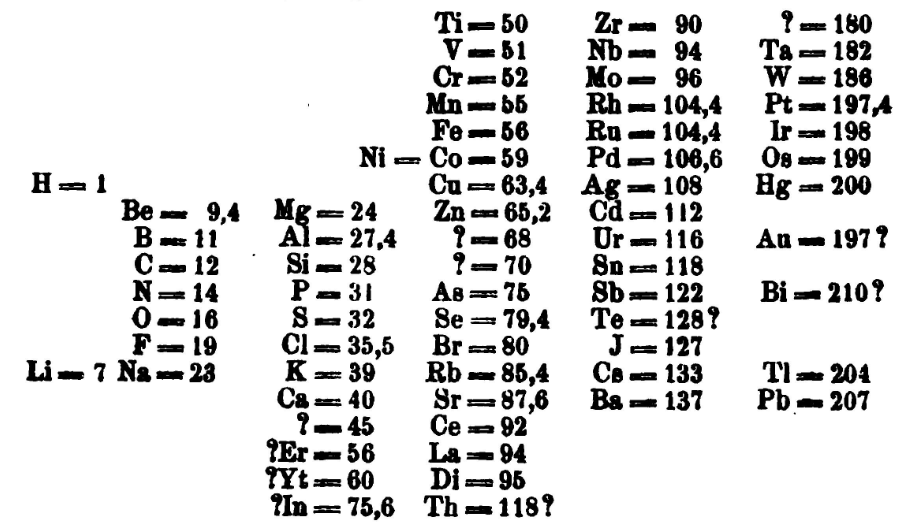
\includegraphics[width=0.7\textwidth]{figures/introduction/PeriodicTable.png}
    \caption{Dimitri Mendeleev's periodic table of elements from the late 1800s, taken from~\cite{MendeleevPaper}. The elements are grouped by similar chemical properties, and the gaps in the table are where Mendeleev predicted that new elements would be discovered.}
    \label{fig:periodic_table}
\end{figure}


Things changed quite a bit around the turn of the 20th century, with scientists like Rutherford and Chadwick determining that the supposedly indivisible atom was composed of even smaller sub-atomic particles, eventually named electrons, protons and neutrons~\cite{Electrons, Protons, Neutrons}. Thus the number of fundamental blocks of matter had decreased substantially from nearly 100 to just three, but only very briefly. Only months after the discovery of the neutron, the fundamental anti-particle of the electron--known as the positron--was discovered in 1932 by Carl Anderson~\cite{Positron}. In the next two decades, the number of known fundamental particles would skyrocket. In 1947, the muon was discovered~\cite{Muon}, followed by the discovery of a laundry list of particles~\cite{Kaon,Lambda,Sigma} that participate in the same interaction that holds oppositely charged protons together in the nucleus of an atom--the so-called \textbf{strong nuclear force}. These ``fundamental'' particles were collectively called \textbf{hadrons}, which were further separated into lighter and heavier categories dubbed \textbf{mesons} and \textbf{baryons}, respectively~\cite{MesonBaryon}. By the late 1960s, the number of known hadrons had grown to well over 100~\cite{ParticleDiscoveries}, which is a far cry from the number of ``fundamental'' chemical elements that were known to exist in the 1800s.

In the same way that Mendeleev tried to group the elements by their similar chemical properties, physicists attempted to group the hadrons together based on their known sub-atomic properties at the time. The first successful attempt at such a grouping was the \textbf{Eightfold Way}, which was independently proposed by Murray Gell-Mann and Yuval Ne'eman in 1961~\cite{GellMannEightfold, NeemanEightfold}. This grouping was found by examining the following properties of the hadrons:
%
\begin{enumerate}
    \item \textbf{Isotopic spin}: a quantum number introduced by Werner Heisenberg in 1932 to try to explain the apparent symmetries between the proton and neutron with respect to the strong nuclear force~\cite{IsotopicSpin} (i.e. although the proton and neutron have different electric charges, the strong interaction does not seem to distiguish between the two)
    \item \textbf{Strangeness}: another quantum number introduced by Gell-Mann and Nishijima in 1953 to explain why some hadrons decayed much more slowly than expected, but such particles appeared to be created in pairs~\cite{Strangeness}. In other words, the strong interaction responsible for the creation of these particles appeared to conserve strangeness, but the weak interaction responsible for the slower decay of these particles did not. This\footnote{Strangeness was introduced a few years before the very first quark model, but it now has the modern interpretation which is directly related to the number of strange and anti-strange quarks within a hadron.} quantity is of utmost importance to this thesis, and will be discussed in much greater detail in the coming sections.
\end{enumerate}
%
\begin{figure}[t!]
    \centering
    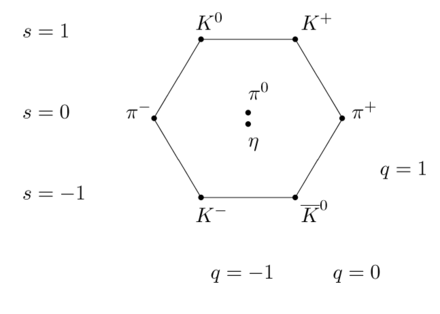
\includegraphics[width=0.49\textwidth]{figures/introduction/Meson_octet.png}
    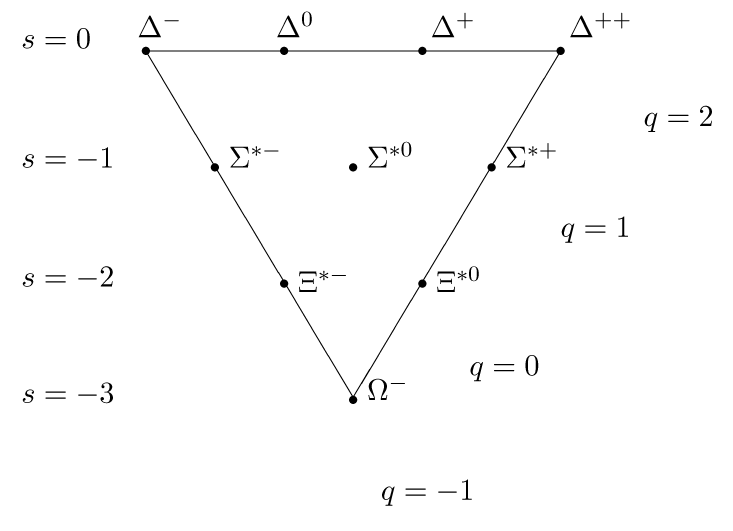
\includegraphics[width=0.49\textwidth]{figures/introduction/Baryon_decuplet.png}
    \caption{The ``Eightfold Way'' diagrams of the J = 1/2 mesons (left) and J = 3/2 baryons (right) plotted against strangeness and electric charge. Understanding the underlying symmetry group that gives rise to such patterns\protect\footnotemark \  ultimately led to the development of the quark model. While the original patterns were found using isotopic spin and hypercharge, it is trivial to convert between the two using the Gell-Mann-Nishijima formula~\cite{GellMannNishijima_1, GellMannNishijima_2}.}
    \label{fig:eightfold_way}
\end{figure}
\footnotetext{Namely SU(3), but this is a history lesson. Also the path from SU(3) to patterns of this type is long and arduous, involving a thorough understanding of representation theory.}
%
Plotting the baryons and mesons in a two-dimensional space based on these two properties revealed striking patterns, as shown in Figure~\ref{fig:eightfold_way}. Similar to Mendeleev, GellMann also left a blank space\footnote{The original paper on the Eightfold Way does not contain any of these diagrams, but there are discussions about the properties of particles that should exist if the theory were correct, but had not been observed~\cite{GellMannEightfold}.} where he believed a new particle--the $\Omega^{-}$--would be discovered.  The patterns in these diagrams hinted at an underlying symmetry governing the strong nuclear force, and ultimately led to the invention of the very first quark model by Gell-Mann and Zweig in 1964~\cite{QuarkModel}. This model proposed that all of the hadrons were actually composed of even smaller particles, which Gell-Mann dubbed ``quarks''. The quark model was able to explain the patterns seen in Figure~\ref{fig:eightfold_way} by introducing three different types of fermionic quarks--up, down and strange--along with their corresponding anti-quarks. Baryons would then be composed of three such quarks, whereas mesons would be composed of quark and anti-quark pairs. If the quark model were correct, the number of fundamental building blocks of matter would again decrease from over 100 to just 14: electrons, muons, electron neutrinos, muon neutrinos, up quarks, down quarks, strange quarks, and all of their corresponding anti-particles.


Initially, many physicists believed that the quarks from this model were just a mathematical abstraction~\cite{QuarkAbstraction}. This possibility did not stop Sheldon Glashow and James Bjorken from extending the quark model in less than a year after its inception by introducing a fourth quark: the charm~\cite{CharmQuark}. This new quark was primarily introduced to equalize the number of leptons (four at the time: electron, muon, and their respective neutrinos) with the number of quarks. The theory was mostly aesthetic~\cite{AestheticCharm} in that the charm quark was not explicity required by any known mechanisms. It was only after the Glashow-Iliopoulos-Maiani (GIM) mechanism was introduced in 1970~\cite{GIM} that the existence of the charm quark became ``necessary''. This mechanism helped explain why neutral kaons decayed into two muons at a much lower rate than expected, but it required the existence of a quark with the same charge as the up quark but with a much larger mass.

On the experimental side of things, the notion that protons and neutrons were fundamental particles was also being challenged. The deep inelastic scattering experiments at the Standford Linear Accelerator Center (SLAC) performed by Kendall, Friedman and Taylor in 1968~\cite{Kendall, Friedman, Taylor} revealed unexpected\footnote{Depending on who you asked at the time, both the three and four quark models were not universally accepted.} behavior when probing the structure of the proton: it appeared to be composed of point-like particles. These experiments were performed by firing electrons at stationary protons and measuring the energy distributions of the scattered electrons at different scattering angles. An example such a distribution for electrons with initial energies of 10 GeV scattered at 6 degrees can be seen in Figure~\ref{fig:dis}. The large spike on the left side of the distribution corresponds to the elastic scattering of the electron off the proton, which was well understood at the time~\cite{ElasticScattering}. The ``bumps'' observed at lower values of the scattered electron energy were also well understood~\cite{Resonances}, and they correspond to the ``shallow'' inelastic scattering of the electron off the proton, where the proton gets excited into a so-called \textit{resonance} state (like the $\Delta$ baryon). However, the ``background'' underneath the bumps and the apparent continuum of events at even lower values of the scattered electron energy correspond to a mess of unknown particles being produced. This mess of particles appeared to grow with increasing scattering angle and decreasing scattered electron energy, which ultimately led to the conclusion that the proton was composed of point-like particles that were being ``knocked out'' of the proton by the incoming electron~\cite{Kendall, BjorkenScaling}.

\begin{figure}[ht]
    \centering
    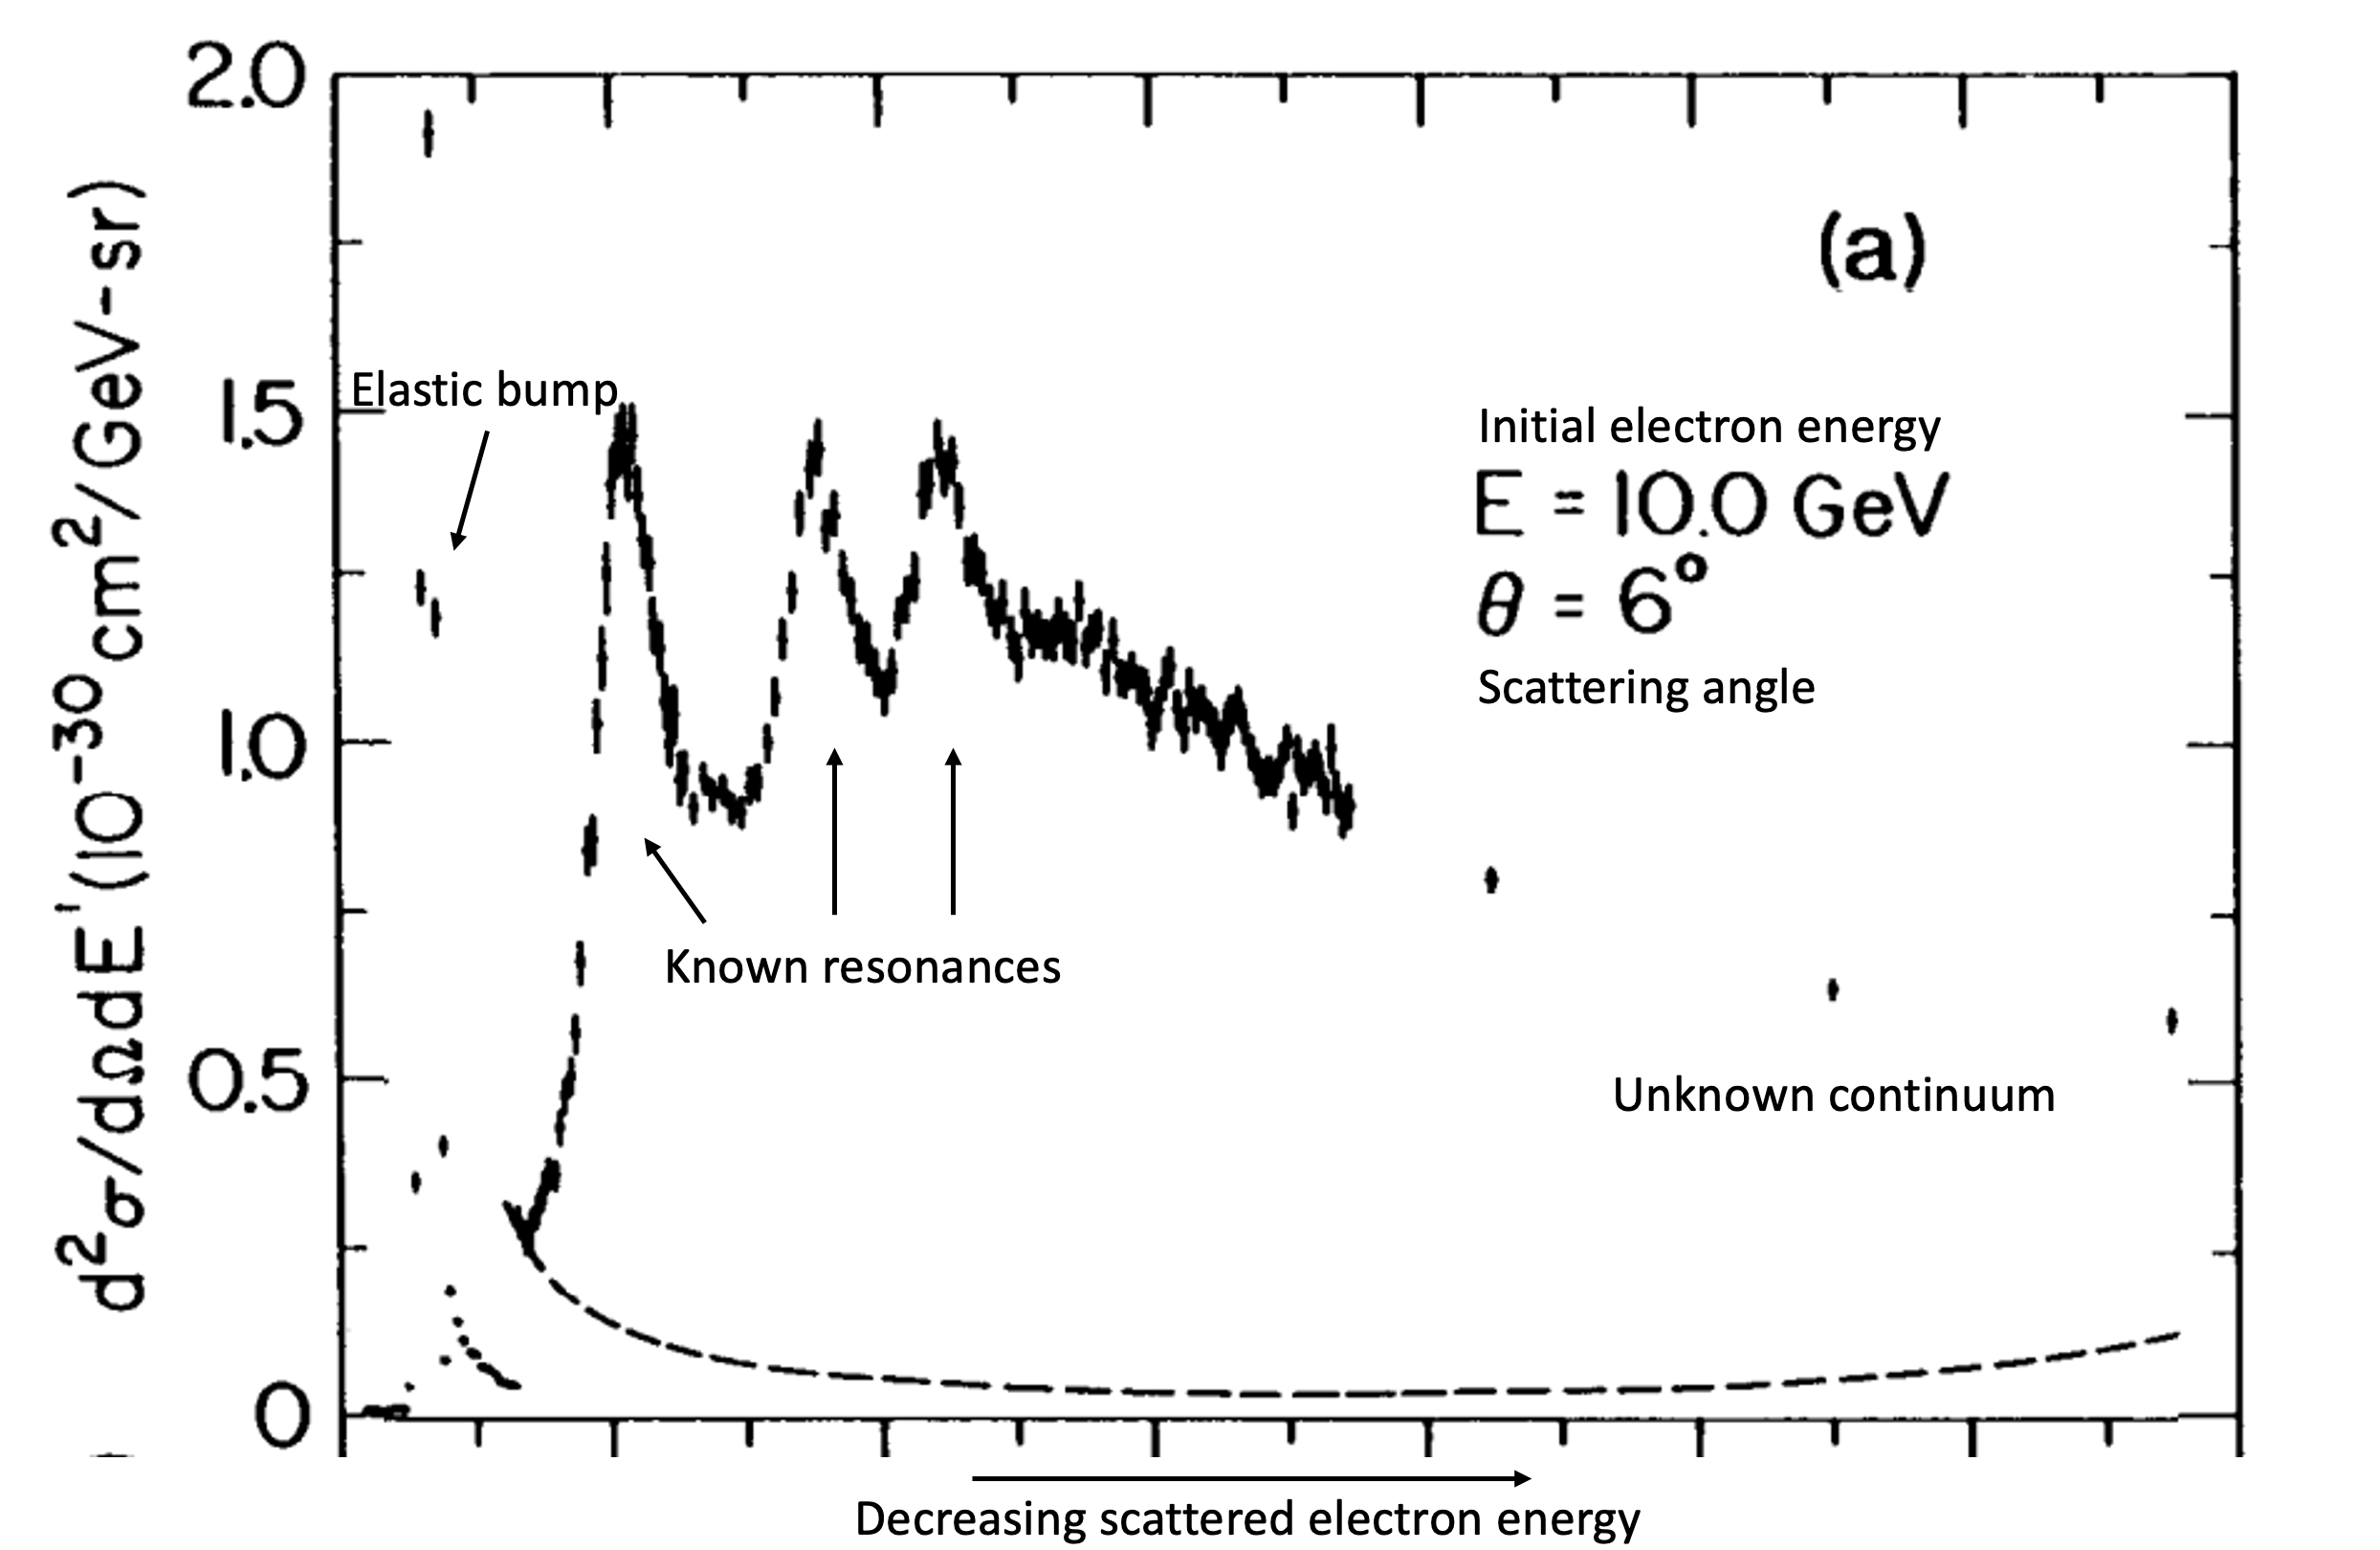
\includegraphics[width=0.7\textwidth]{figures/introduction/DeepInelasticScattering.png}
    \caption{The energy distribution of electrons scattered off of protons at an initial electron energy of 10 GeV and a scattering angle of 6 degrees. The large spike on the left side of the distribution corresponds to the elastic scattering of the electron off the proton, and the ``bumps'' correspond to the inelastic scattering of the electron off the proton. The ``background'' underneath the bumps and the apparent continuum of events at even lower values of the scattered electron energy correspond to a mess of unknown particles being produced. The behavior of this continuum with respect to the scattering angle and the scattered electron energy ultimately led to the conclusion that the proton was not fundamental.}
    \label{fig:dis}
\end{figure}

While many physicists were perfectly happy to interpret these point-like particles as the very same quarks from the aforementioned quark model(s), they received the much more noncommittal name \textbf{partons} after Richard Feynman's parton model of hadrons~\cite{Partons}. The association of these partons with quarks was not universally accepted\footnote{No acceptance of any model is a step function, but the discovery of J/$\psi$ seems to be a turning point in literature.} until the discovery of the J/$\psi$ meson in 1974~\cite{Jpsi}. In the meantime, the theoretical description of the strong nuclear force was closing in on its final form. The formulation of Quantum ChromoDynamics (QCD) in the early 1970s by Gell-Mann, Fritzsch, and Leutwyler~\cite{QCDFormulation} resolved many of the issues that were present in the initial quark models\footnote{For example, the wavefunction of the $\Delta^{++}$ baryon under the first quark model was not anti-symmetric, which is a requirement for fermions.}. QCD introduced the concept of color charge, which all of the quarks would carry. The mediating bosons of the strong interaction--known as \textbf{gluons}--were also introduced\footnote{And also carried color charge, but more details will be discussed in Section~\ref{sec:qcd}}. 

While QCD gave a solid mathematical description of the strong interaction, it wasn't until the discovery of \textbf{asymptotic freedom}~\cite{AssFreedom1, AssFreedom2} by Gross, Wilczek and Politzer in 1973 that the theory became experimentally testable. Asymptotic freedom is the notion that the strong interaction becomes weaker at higher energies, allowing for QCD calculations to be performed using perturbative techniques. This discovery allowed theorists to use QCD to make predicitions of the results of very high energy particle collision experiments. The first QCD prediction to be experimentally verified came from the Positron-Electron Tandem Ring Accelerator (PETRA) in 1979~\cite{PETRA}, which experimentally confirmed the existence of gluons~\cite{GluonConfirmation}. With experimental verification of QCD, it became clear that the association of partons with quarks was indded incorrect: they are both quarks \textit{and} gluons.

While not of particular import to this thesis\footnote{Though extremely interesting in its own right}, the theory of electroweak interactions was also being developed during the 1960s by Glashow, Weinberg and Salam~\cite{Electroweak1, Electroweak2}. With this new theory came the prediction of four\footnote{The Higgs mechanism (which predicts the existence of the Higgs boson) came before electroweak unification~\cite{HiggsPaper}, but it was a requirement for the theory.} new bosons: the Higgs boson, the charged W$^{\pm}$ bosons, and the neutral Z$^{0}$ boson. With the combined theories of the electroweak and strong interaction, the \textbf{Standard Model} of particle physics--which describes the now 61\footnote{There are many ways to count fundamental particles, but this particular number is obtained by: 6 leptons ($\times 2$ for anti-leptons), 6 quarks ($\times 3$ for each color, $\times 2$ for anti-quarks), 1 gluon ($\times 8$ for color), 1 photon, the W and Z bosons, and the Higgs boson. The more common number of seventeen~\cite{ParticleNumber} is a bit low, especially given that anti-particles have already been counted in the earlier parts of this section.} fundamental particles and how they interact--was complete. 


\section{The Standard Model}

Before diving into some details regarding the Standard Model, a few reminders will be given.

\subsection{Lagrangian formalism}

\subsection{Fields}

\subsection{Symmetries}

\subsection{Famous equations}

\subsection{The Standard Model Lagrangian}

\section{Quantum Chromodynamics}
\label{sec:qcd}

This section serves as a turning point for this thesis: while the discussions above have been \textit{mostly} general, the novel research presented in this thesis is centered around the strong nuclear force. As such, the remainder of this chapter will delve into the details of this mysterious force, and how it can be studied using high-energy particle collisions. 

The quantum field theory which describes the interaction between quarks and gluons--generally referred to as the strong interaction or strong nuclear force--is known as \textbf{Quantum ChromoDynamics} (QCD). In this theory, the quarks and gluons have an additional quantum number known as \textbf{color charge}, which is (somewhat) analagous to the electric charge in Quantum ElectroDynamics (QED). 


\subsection{The QCD Lagrangian}
\label{sec:qcd_lagrangian}

As discussed in Section~\ref{sec:lagrangian_formalism}, the main tool for investigating the dynamics of a quantum field theory is through its Lagrangian. In principle, the QCD Lagrangian has already been introduced: it is completely contained within the Standard Model Lagrangian given in Equation~\ref{eq:sm_lagrangian}. However, when the only theory of interest is that of the strong interaction, the electroweak gauge fields, leptons and scalars can be dropped to give only the QCD Lagrangian~\cite{QCDLagrangian},
%
\begin{align*}
    \label{eq:qcd_lagrangian}
    \mathcal{L}_{Q C D}= & -\frac{1}{4} F_{\mu \nu}^A F^{A \space \mu \nu}+i \bar{q} \gamma^\mu\left(\partial_\mu+i g_s \frac{1}{2} \lambda^A \mathcal{A}_\mu^A\right) q \\
    & -\bar{q}_{\mathrm{R}} \mathcal{M} q_{\mathrm{L}}-\bar{q}_{\mathrm{L}} \mathcal{M}^{\dagger} q_{\mathrm{R}}-\theta \omega,
\end{align*}
%
where all repeated indices are summed over.

The gluons are described by the vector gauge field $\mathcal{A}_\mu^A$, with index $A$ representing one of the eight color labels. These eight components belong to the color group SU$_\text{c}$(3), which is the gauge group of QCD. The corresponding field strength tensor $F_{\mu \nu}^A$ is given by
%
\begin{equation}
    \label{eq:field_strength_tensor}
    F_{\mu \nu}^A = \partial_\mu \mathcal{A}_\nu^A - \partial_\nu \mathcal{A}_\mu^A + g_s f^{ABC} \mathcal{A}_\mu^B \mathcal{A}_\nu^C,
\end{equation}
%
where $f^{ABC}$ are the structure constants~\cite{StructureConstants} of SU$_\text{c}$(3). Note that while this field strength tensor shares the same letters as the electromagnetic field strength tensor $F_{\mu \nu}$, the additional term $g_s f^{ABC} \mathcal{A}_\mu^B \mathcal{A}_\nu^C$ in Equation~\ref{eq:field_strength_tensor} separates QCD and QED in a very fundamental way: the gluons are allowed to self-interact. This self-interaction is a direct result of the non-vanishing structure constants of SU$_\text{c}$(3)\footnote{Structure constants of Abelian gauge groups like U(1) are trivially zero.}, and causes a lot of headaches for theorists. 

The quarks are represented by the field $q$, which is a bit misleading as the color, flavor and spin indices have been suppressed. In reality, the quark field $q$ has:
%
\begin{itemize}
    \item six flavor indices $\{u, d, s, c, b, t\}$,
    \item four spin indices $\{0, 1, 2, 3\}$, and
    \item three color indices $\{r, g, b\}$,
\end{itemize}
%
where all of these indices are being implicitly summed over in $\mathcal{L}_{QCD}$. Luckily all of the matrices ($\mathcal{A}_\mu^A, \lambda^A, \mathcal{M}, \gamma^\mu$) act on separate sets of indices. For example, the $\gamma^\mu$s only operate on the spin indices, whereas both $\mathcal{A}_\mu^A$ and $\lambda^A$ operate on the color indices.

The chiral quark fields $q_\text{L}$ and $q_\text{R}$ are defined as $\frac{1}{2}(1 - \gamma_5)q$ and $\frac{1}{2}(1 + \gamma_5)q$, respectively.  



\subsubsection{Why eight gluons?}
\label{sec:why_eight_gluons}

The gluon field $\mathcal{A}^A$ transforms under the adjoint respresentation of SU(3), which is a representation of SU(3) on the vector space of its Lie algebra $\mathfrak{su}(3)$. As $\mathfrak{su}(3)$ has eight basis elements (for instance, the Gell-Mann matrices $\lambda^A$ from above), the adjoint representation of SU(3) is eight-dimensional. Thus the gluon field has eight independent components, or there are eight gluons.

This is why representation theory is so fun: the term $g_s f^{ABC} \mathcal{A}^B \mathcal{A}^C$  can be thought of as boring $3\times3$ matrix multiplication, but it can also be thought of as an inner product between two eight-dimensional vectors. Unfortunately the fun breaks down at some point, as terms like $i \bar{q} \gamma^\mu (i g_s \frac{1}{2} \lambda^A \mathcal{A}_\mu^A) q$  can only be intepreted as $\mathcal{A}$ transforming $q$ under the fundamental representation of SU(3) (i.e. $3\times3$ matrix acting on $3\times1$ vector). Furthermore, writing $\lambda^A$ as an $8\times8$ matrix is not particulalry enlightening--though it can be done. For example, $\lambda^1$ in the adjoint represntation is given by
%
\begin{equation*}
\lambda^{1, \text {adjoint }}=\left(\begin{array}{cccccccc}
0 & 0 & 0 & 0 & 0 & 0 & 0 & 0 \\
0 & 0 & -2i & 0 & 0 & 0 & 0 & 0 \\
0 & 2i & 0 & 0 & 0 & 0 & 0 & 0 \\
0 & 0 & 0 & 0 & 0 & 0 & -i & 0 \\
0 & 0 & 0 & 0 & 0 & i & 0 & 0 \\
0 & 0 & 0 & 0 & -i & 0 & 0 & 0 \\
0 & 0 & 0 & i & 0 & 0 & 0 & 0 \\
0 & 0 & 0 & 0 & 0 & 0 & 0 & 0
\end{array}\right),
\end{equation*}
which is found by interpreting the commutation relation $[\lambda^{1, \text {adjoint}}, \lambda^A] = 2if_{1AB}\lambda^B$ as the action of $\lambda^{1, \text {adjoint }}$ on $\lambda^A$, where each $\lambda^A$ is assigned to a trivial column vector with a $1$ and the $A^{\text {th}}$ index and zeroes everywhere else.

In principle, QCD could have been built on top of a U(3) gauge group, which would give rise to nine gluons (as the dimension of U(n) is $n^2$). However, the singlet state in U(3) must not be interacting: if it were, color neutral baryons would interact with each other via the strong interaction at a much longer range~\cite{SingletGluons}. As there is no physical difference between U(3) with a non-interacting singlet and SU(3), the simpler gauge group was chosen. 

%





